\documentclass[main_dicodile]{subfiles}
\begin{document}


\section{Locally greedy Coordinate Descent}
\parttitleframe{Moreau2018}


% Intro section
\begin{frame}[t]
%\vskip-1em
\frametitle{$Z$-step: Sparse coding}
$\rightarrow \pmb D$ fixed, update $Z$
\[
Z^{[n],*} = \argmin_{Z^{[n]}}\| X^{[n]} - \sum_{k=1}^K\pmb D_k *  Z_k^{[n]}\|_2^2
+ \lambda\| Z^{[n]}\|_1
\]
\strongpoint{Independent for each $n\in\llbracket1, N\rrbracket$}
\vskip1em
%
\underline{\textbf{Related Algorithms:}}\\[.5em]
\begin{itemize}%\itemsep.5em
    \item Iterative Soft-Thresholding Algorithm (ISTA)\\\mycite{Daubechies2004, Chalasani2013}
    \item Fast ISTA \\\mycite{Beck2009, Wohlberg2016}
    \item Alternated Direction Method of Multiplier (ADMM)\\\mycite{Gabay1976, Bristow2013}
    \item Coordinate Descent (CD) \\\mycite{Friedman2007, Kavukcuoglu2013}
\end{itemize}
\end{frame}


\begin{frame}{Complexity Summary}

\begin{itemize}\itemsep1em
    \item Full gradient methods: $\bO{\frac{K^2TL}{\epsilon}}$
    \begin{itemize}
        \item[$\triangleright$] Iteration complexity with pre-computation : $\bO{K^2TL}$
        \item[$\triangleright$] Convergence in $\bO{\frac{1}{q}}$
    \end{itemize}
    \item Coordinate Descent: $\bO{\frac{K^2TL}{\epsilon}}$
    \begin{itemize}
        \item[$\triangleright$] Iteration complexity with pre-computation : $\bO{KL}$
        \item[$\triangleright$] Convergence in $\bO{\frac{1}{qTK}}$
    \end{itemize}

    \strongpoint{Does not seem to be much to gain using CD.}
    
    \vskip1em
    But the convergence rate could be pessimistic for CD...\\
    If the updates are performed on the "right" coefficients, the cvg rate becomes $\bO{\frac{1}{qS}}$ where $S$ is the number of non-zero in $Z^*$.
\end{itemize}

\end{frame}


%---------------------------------------------------------------------------
\subsection{LGCD}
%---------------------------------------------------------------------------

\begin{frame}[t]{Coordinate Descent (CD)}
	
	Minimize
    %
	\[
    	Z^{*} = \argmin_{Z}\| X - \sum_{k=1}^K\pmb D_k *  Z_k\|_2^2
    			+ \lambda\| Z\|_1
	\]
    %
	Update one coordinate at each iteration.\\[1em]
	\begin{enumerate}
		\item Select a coordinate $(k_0, \omega_0)$ to update.
		\visible<2->{ \item Compute a new value $Z'_{k_0}[\omega_0]$ for this coordinate}
	\end{enumerate}

\only<1>{
	Three algorithms for LASSO:
	\begin{itemize}\itemindent1em
		\item Cyclic updates; $\bO{1}$  \mycite{Friedman2007}
		\item Random updates; $\bO{1}$ \mycite{Nesterov2010}
		\item Greedy updates; $\bO{KT}$ \mycite{Osher2009}
	\end{itemize}
}
\only<2>{
	For convolutional CD, we can use optimal updates:
	$$
		Z'_{k_0}[\omega_0] = \frac{1}{\|\pmb D_{k_0}\|_2^2}
        \textbf{ST}(\beta_{k_0}[\omega_0], \lambda),
	$$
	with {\small $\textbf{ST}(y, \lambda) = \text{sign}(y)(|y| - \lambda)_+$}.
	\cite{Kavukcuoglu2013} showed this can be done efficiently, with $\mathcal O(KL)$ operations.
}
\only<3>{
    \strongpoint{Converges to an optimal point for CSC problem with rate $\bO{\frac{1}{q}}$.
}
    
    \vskip1em
    Trade-off between cheap computational complexity (random/cyclic CD) and importance sampling with faster convergence (Greedy CD).\\\mycite{Nutini,Karimireddy2018}
}
\end{frame}




\begin{frame}{Locally Greedy Coordinate Descent \citeconfright{Moreau2018}{ICML}}


We introduced the LGCD method which is an extension of GCD.\\
{
    \centering
    \inputTikZ{.7}{LGCD}
}

\only<1-2>{
    \vskip1em
    GCD has $\mathcal O(K{T})$ computational complexity.\\[1em]
    \only<2>{But the update itself has complexity $\mathcal O(KL)$}
}
%
\visible<3->{
    With a partition $\mathcal C_m$ of the signal domain $[1, K]\times [0, {T}[$,
    \[
    \mathcal C_m = [1, K]\times [\frac{(m-1){T}}{M}, \frac{m{T}}{M}[
    \]%
}%
\visible<4->{%
    The coordinate to update is chosen greedily on a sub-domain $\mathcal C_m$\\[1em]
    
    {\centering$\frac{{T}}{M} = 2L-1~~\Rightarrow~~\mathcal O$(Coordinate selection) = $\mathcal O$(Coordinate Update)\\[1em]}
    
    The overall iteration complexity is $\mathcal O(KL)$ instead of $\mathcal O(K{T})$.
    \strongpoint{Efficient for sparse $Z$}
}


\end{frame}

\begin{frame}{Fast optimization}
Comparison of the coordinate selection strategy for CD on simulated signals\\
We set $K=10$, $L=150$, $\lambda = 0.1 \lambda_{\max}$\\[1em]
\centering
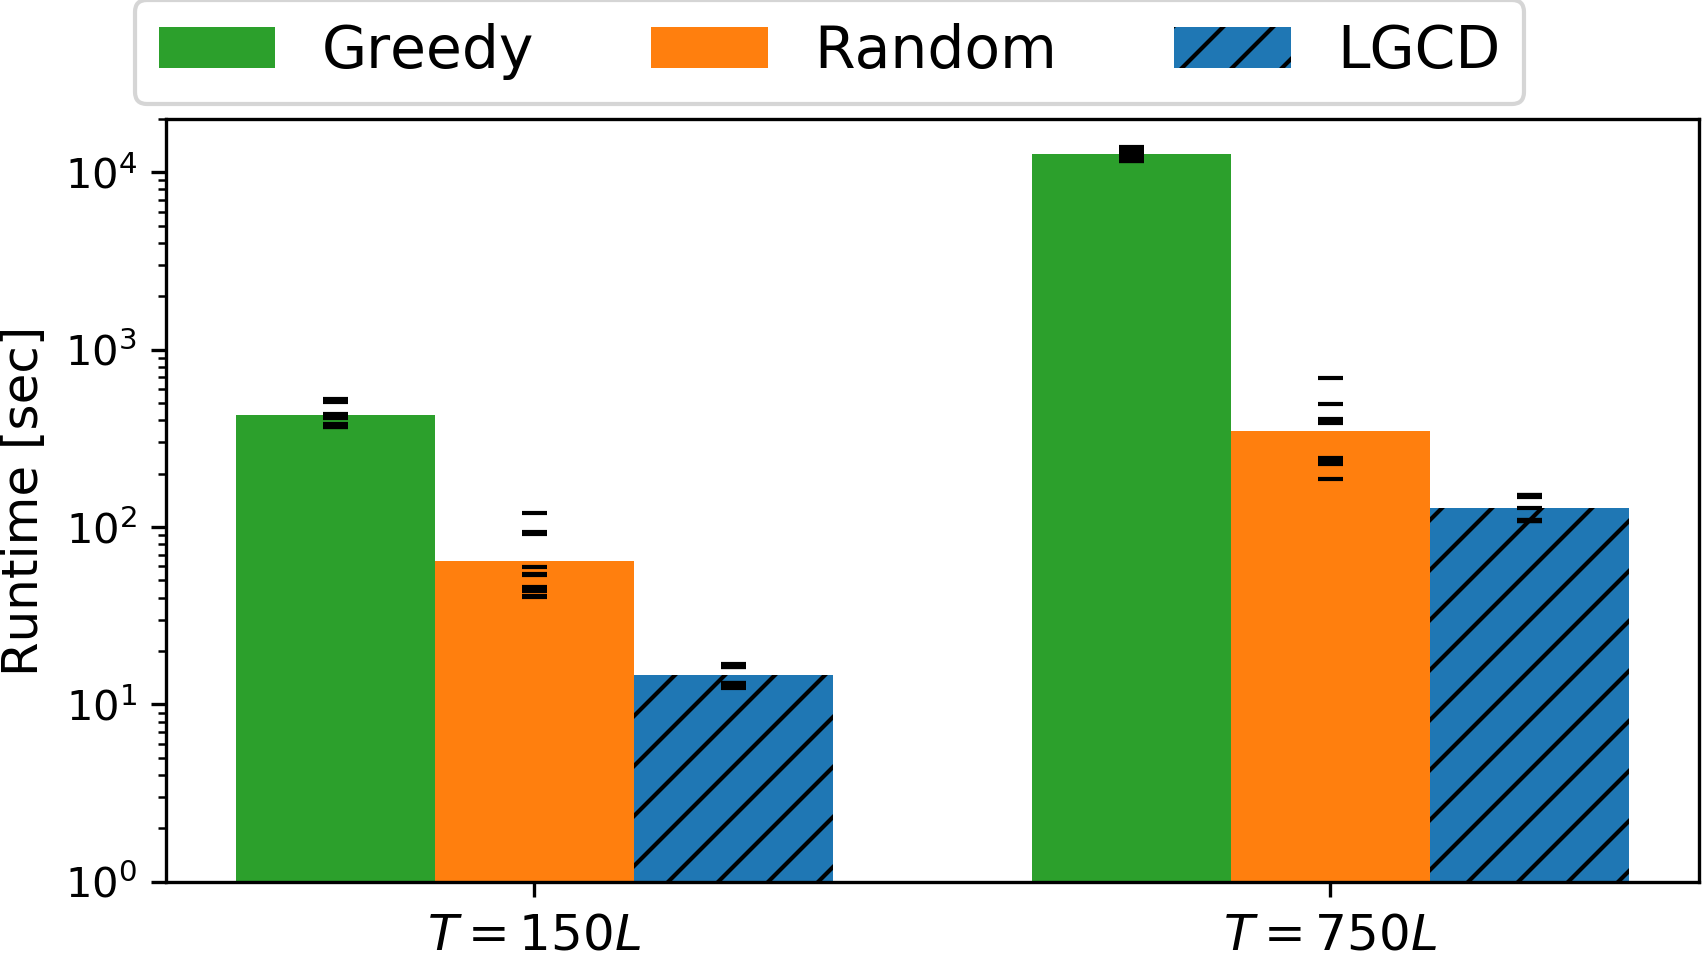
\includegraphics[width=.9\textwidth]{CD_strategies_comparison.png}
\end{frame}


\begin{frame}{Comparison with full batch method}
    \alt<2>{
        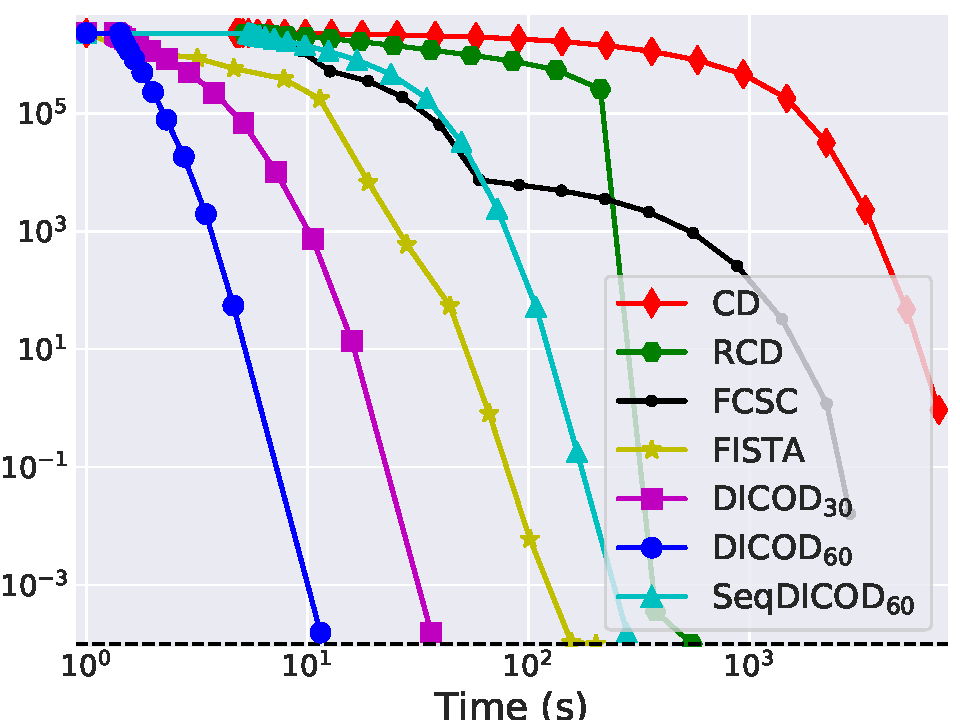
\includegraphics[width=.9\textwidth]{cost_curve_seaborn_time_small}
    }{
        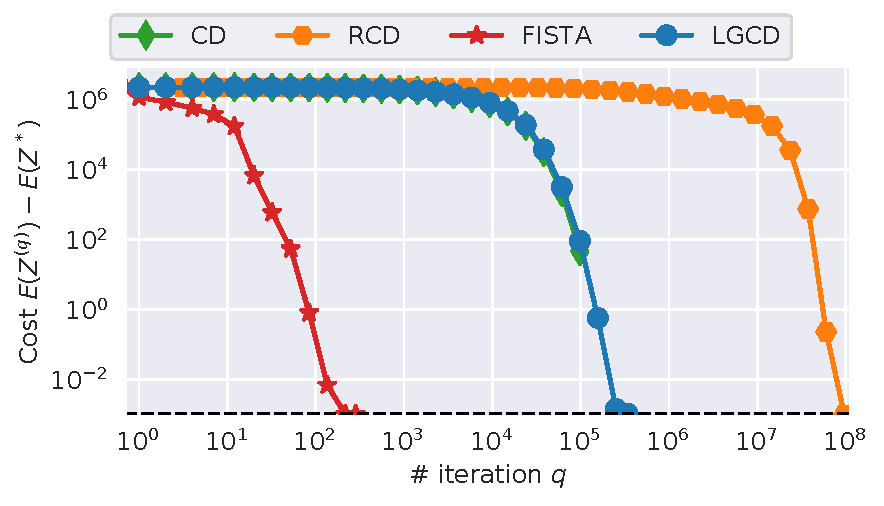
\includegraphics[width=.9\textwidth]{cost_curve_seaborn_iter_small}
    }
\end{frame}


%---------------------------------------------------------------------------
\section{Distributed algorithm for sparse coding:\\
         DICOD and DiCodile-Z}
%---------------------------------------------------------------------------
\parttitleframe{}

\begin{frame}{Weak dependence of the coordinate updates}
The update of the $W$ coordinates $(k_w, \omega_w)_{w=1}^W$ with additive update $\Delta Z_{k_w}[\omega_w]$ changes the cost by:
\begin{align*}
\Delta E =
\overbrace{\sum_{i=1}^W\Delta E_w}^{
    \text{iterative steps}}
- \underbrace{\sum_{w \neq w'}(\pmb D_{k_w} * \pmb D_{k_{w'}}^\Lsh)[\omega_{w'} - \omega_w]
    \Delta Z_{k_w}[\omega_w] \Delta Z_{k_{w'}}[\omega_{w'}]}_{
    % \Delta Z_{k_w}[w] \Delta Z_{k_{w'}}[w']}_{
    \text{interference}}, \label{eq:interf}
\end{align*}

\strongpoint{If the updates are far enough, they can be considered as independent.}
\end{frame}

\begin{frame}{Distributed Convolutional Coordinate Descent\\\citeconfright{Moreau2018}{ICML}}

{
\centering
\inputTikZ{.7}{DICOD}\\
}
\vskip1em
\begin{itemize}[<+->]\itemsep1em
\item Split the coordinates in continuous sub-segment
$\mathcal S_w = \left[\frac{(w-1)T}{W}, \frac{wT}{W}\right[$.
\item Use Greedy CD updates in parallel in each sub-segment.
\item Notify neighbor workers when the update is on the border of $\mathcal S_w$.
\item What do we do when two updates are interfering?
\end{itemize}

\end{frame}



\begin{frame}{DICOD convergence \citeconfright{Moreau2018}{ICML}}
\setbeamercolor{my title}{bg=primary!60, fg=secondary}
\setbeamercolor{my body}{bg=white, fg=black}

DICOD converges to the solution of the CSC for 1D signals without having a control mechanism on the interference.\\[1em]

\begin{beamerboxesrounded}[upper=my title,lower=my body,shadow=true]{
        \usebeamerfont{block title}Theorem (Convergence of DICOD)}
    We consider the following assumptions:\\[.3em]
    {\bf H1: }
    If the cross correlation between atoms of $\pmb D$ is strictly smaller than 1.\\[.3em]
    {\bf H2: }
    No cores stop before all its coefficients are optimal.\\[.3em]
    {\bf H3: }
    If the delay in communication between the processes is inferior to the update time.\\[1em]
    Under these assumptions, the DICOD algorithm converges asymptotically to the
    optimal solution $Z^*$ of CSC.
\end{beamerboxesrounded}

\end{frame}

\begin{frame}{Distributed Convolutional Dictionary Learning (DiCoDiLe-Z)\\\citeconfright{Moreau2019}{preprint}}

\begin{columns}[c]
    \column{.5\textwidth}
    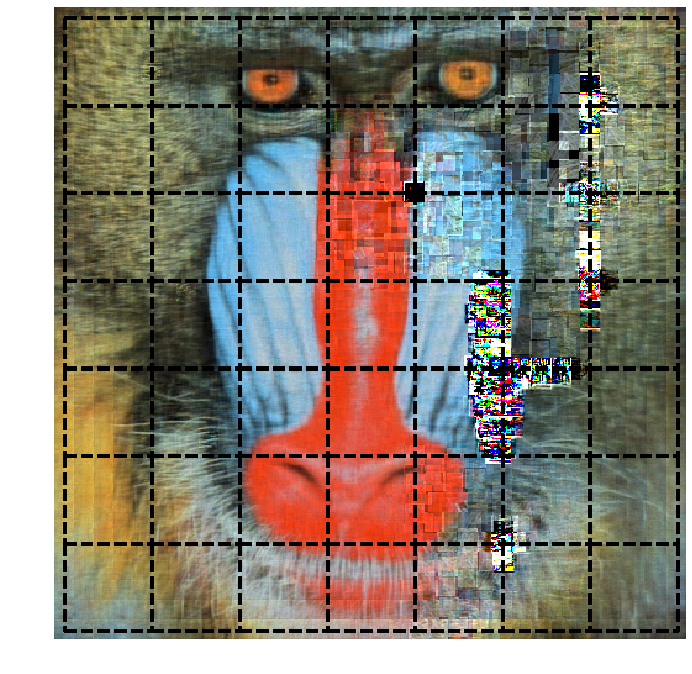
\includegraphics[width=.9\textwidth]{without_soft_lock_M49_support16}
    \column{.5\textwidth}
    \begin{itemize}[<+->]\itemsep1em
        \item DICOD does not work for higher dimensional signals.
        \item Extension require to control interference with more than 2 workers. 
        \item Use asynchronous mechanism: Soft-lock.
    \end{itemize}
\end{columns}

\end{frame}




\begin{frame}[t]{Soft-Locks \mycite{Moreau2019}}
\vskip2em
{
    \centering
    \inputTikZ{.7}{soft_lock}\\
}

\begin{itemize}[<+->]
    \item Keep track of the value of the optimal update in an extended zone of size $L-1$.
    \item Select an update candidate with LGCD.
    \item If it is in the interfering zone, compare the value of the update with the value potential updates in the other worker.
    \item Only perform the udpate if it is larger than the other update.
\end{itemize}

\only<5>{\strongpoint{Give an update order asynchronously.}}

\end{frame}

\begin{frame}{Distributed Convolutional Dictionary Learning (DiCoDiLe-Z)\\\citeconfright{Moreau2019}{preprint}}

\begin{columns}[c]
    \column{.5\textwidth}
    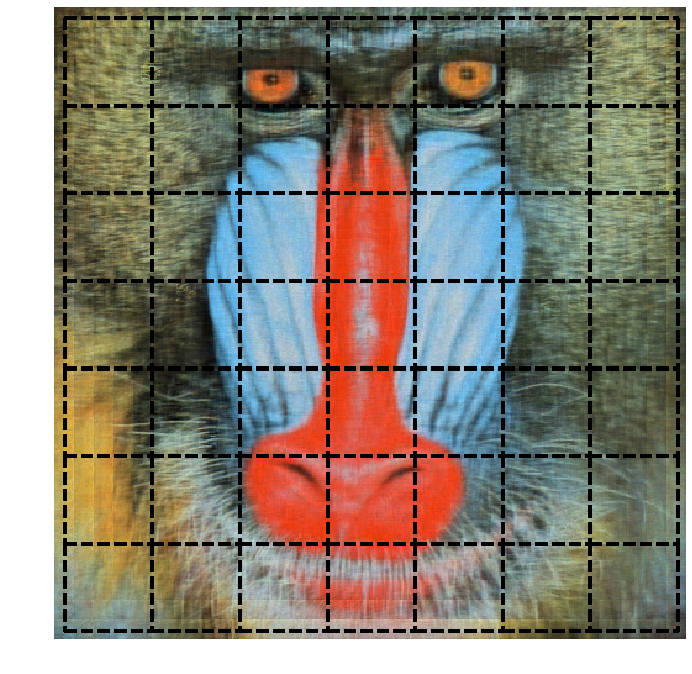
\includegraphics[width=.9\textwidth]{with_soft_lock_M49_support16}
    \column{.5\textwidth}
    \begin{itemize}\itemsep1em
        \item DICOD does not work for higher dimensional signals.
        \item Extension require to control interference with more than 2 workers. 
        \item Use asynchronous mechanism: Soft-lock.
    \end{itemize}
\end{columns}

\end{frame}


\begin{frame}{Numerical speed-up}

\centering
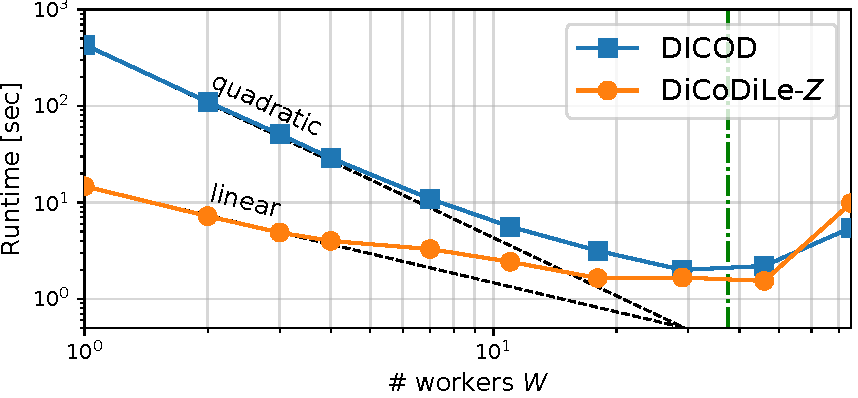
\includegraphics[width=\textwidth]{scaling_T150}
\\
\large Running time as a function of the number of workers $W$.

\end{frame}


\begin{frame}{Scaling on a grid}

\centering
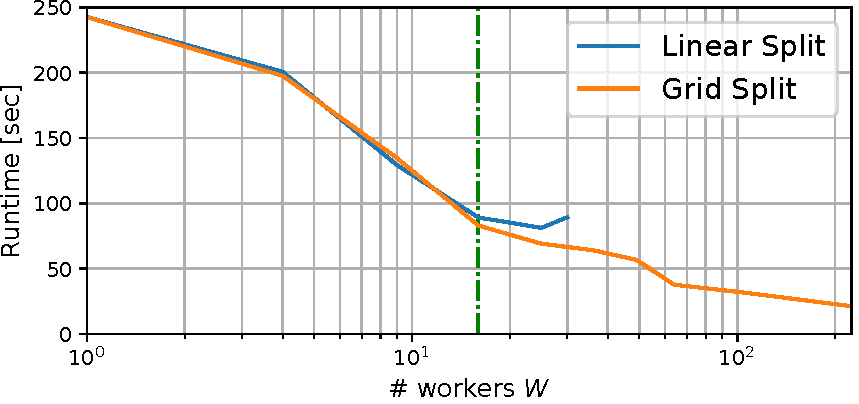
\includegraphics[width=\textwidth]{scaling_grid}
\\
\large Running time as a function of the number of workers $W$.

\end{frame}



\section{Leveraging distributed computation for\\
    dictionary updates}
\parttitleframe{}


\begin{frame}{D-step: solving for the atoms}

The dictionary update is performed by minimizing
\begin{equation}
\min_{\|\pmb D_{k}\|_2 \leq 1} E(\pmb D) \overset{\Delta}{=} \sum_{n=1}^N\frac{1}{2}\|X^n - \sum_{k=1}^K z^n_k * \pmb D_k\|_{2}^{2} \hspace{6pt}
\enspace .
\end{equation}

Computing $\nabla_{\pmb D_k} E(\pmb D)$ can be done efficiently
\[
\nabla_{\pmb D_{k}} E(\pmb D)
= \sum_{n=1}^N (z_k^n)^\Lsh * \left(x^n - \sum_{l=1}^K z^n_l * \pmb D_l\right)
=  \Phi_k - \sum_{l=1}^K \Psi_{k, l} *  \pmb D_l \enspace ,
\]

\strongpoint{Save with Projected Gradient Descent (PGD) with an Armijo backtracking line-search for the D-step \mycite{Wright1999}.}

\vskip1em
However, the computation of $\Psi$ and $\Phi$ can be costly.

\end{frame}

\begin{frame}{Constant computation \mycite{Moreau2019}}

As each worker is handeling a disjoint sub-domain $\mathcal S_w$ of the signal domain $\Omega$ such that $\displaystyle\cup_{w=1}^W\mathcal S_w = \Omega$,
    \begin{align*}
    %\label{eq:phi}
    \Psi_{k,l}[\tau] &= Z_k^\Lsh * Z_l[\tau]
      = \sum_{\omega\in\Omega} Z_k[\omega]Z_l[\tau + \omega]\\
    & = \sum_{w=1}^W \sum_{\omega\in\mathcal S_w} Z_k[\omega]Z_l[\tau + \omega]
    \end{align*}
    \begin{align*}
    %\label{eq:psi}
    \Phi_{k}[\tau] &= Z_k^\Lsh * X[\tau]
        = \sum_{w=1}^W \sum_{\omega\in\mathcal S_w} Z_k[\omega]X[\tau + \omega]
    \end{align*}
    
    \strongpoint{Computational cost is $\bO{K(K+P)L(\frac{T}{W} + WL)}$}
\end{frame}


\section{Numerical Experiments}
\parttitleframe{}

\begin{frame}{Comparition with distributed CDL}
    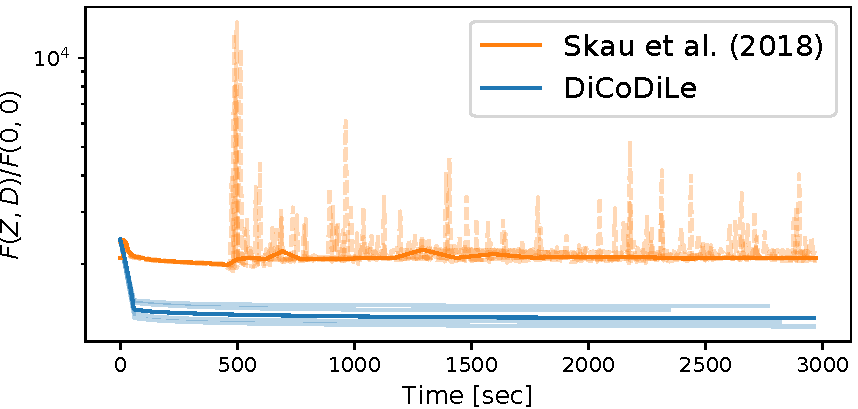
\includegraphics[width=.9\textwidth]{compare_cdl}
\end{frame}

{
    \usebackgroundtemplate{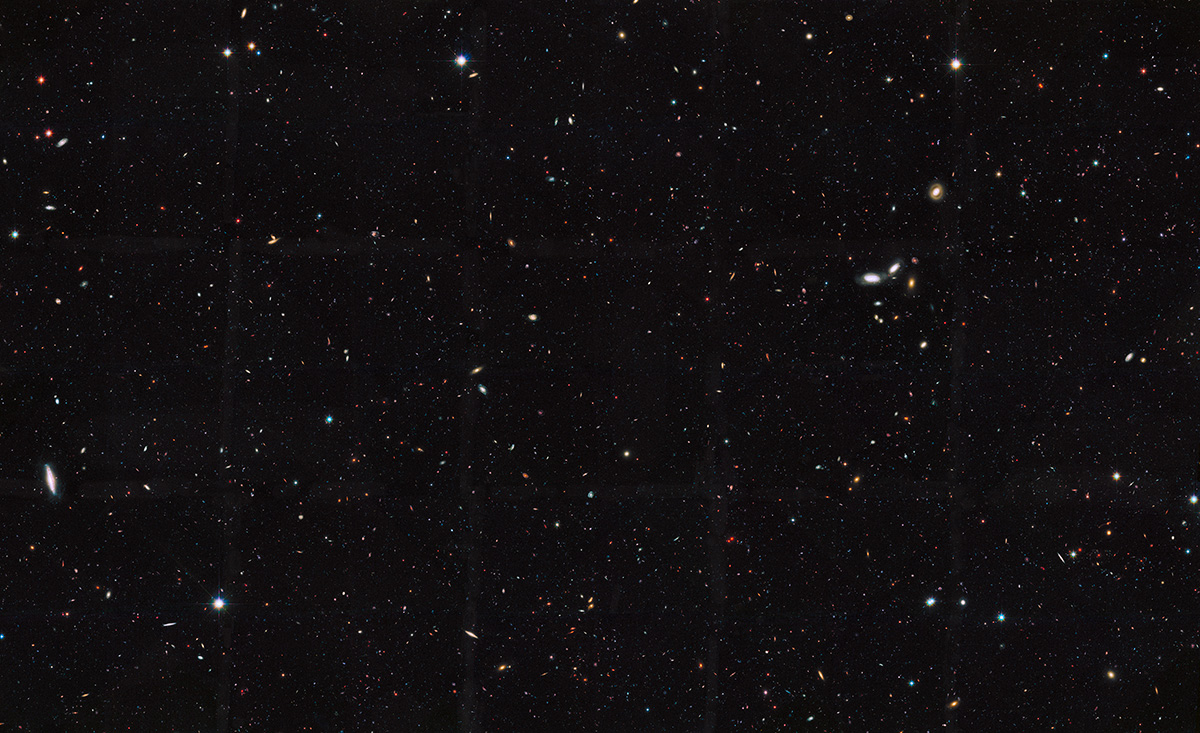
\includegraphics[height=\paperheight]{STScI-H-2016-39-a-Small}}%
\begin{frame}{Images from Hubble Space Telescope}


\setbeamercolor{HST title}{bg=primary!60, fg=title}
\setbeamercolor{HST body}{bg=white, fg=black}

\begin{center}

    \only<2>{
        \begin{minipage}{.6\textwidth}
        \begin{beamerboxesrounded}[
            upper=title,lower=body,shadow=false]{
                \usebeamerfont{block title}\bf Hubble Space Telescope GOODS}
                \vskip-.5em
                \begin{beamercolorbox}[wd=1.04\textwidth]{separation line}\rule{0pt}{2pt}\end{beamercolorbox}\vfill
            \begin{itemize}
                \item Resolution $6000\times 3600$
                \item $K=25$ with atoms of size $32\times 32$
                \item $\lambda = 0.1 \lambda_{\max}$
            \end{itemize}
        \end{beamerboxesrounded}
        \end{minipage}
    }
    \only<3>{
        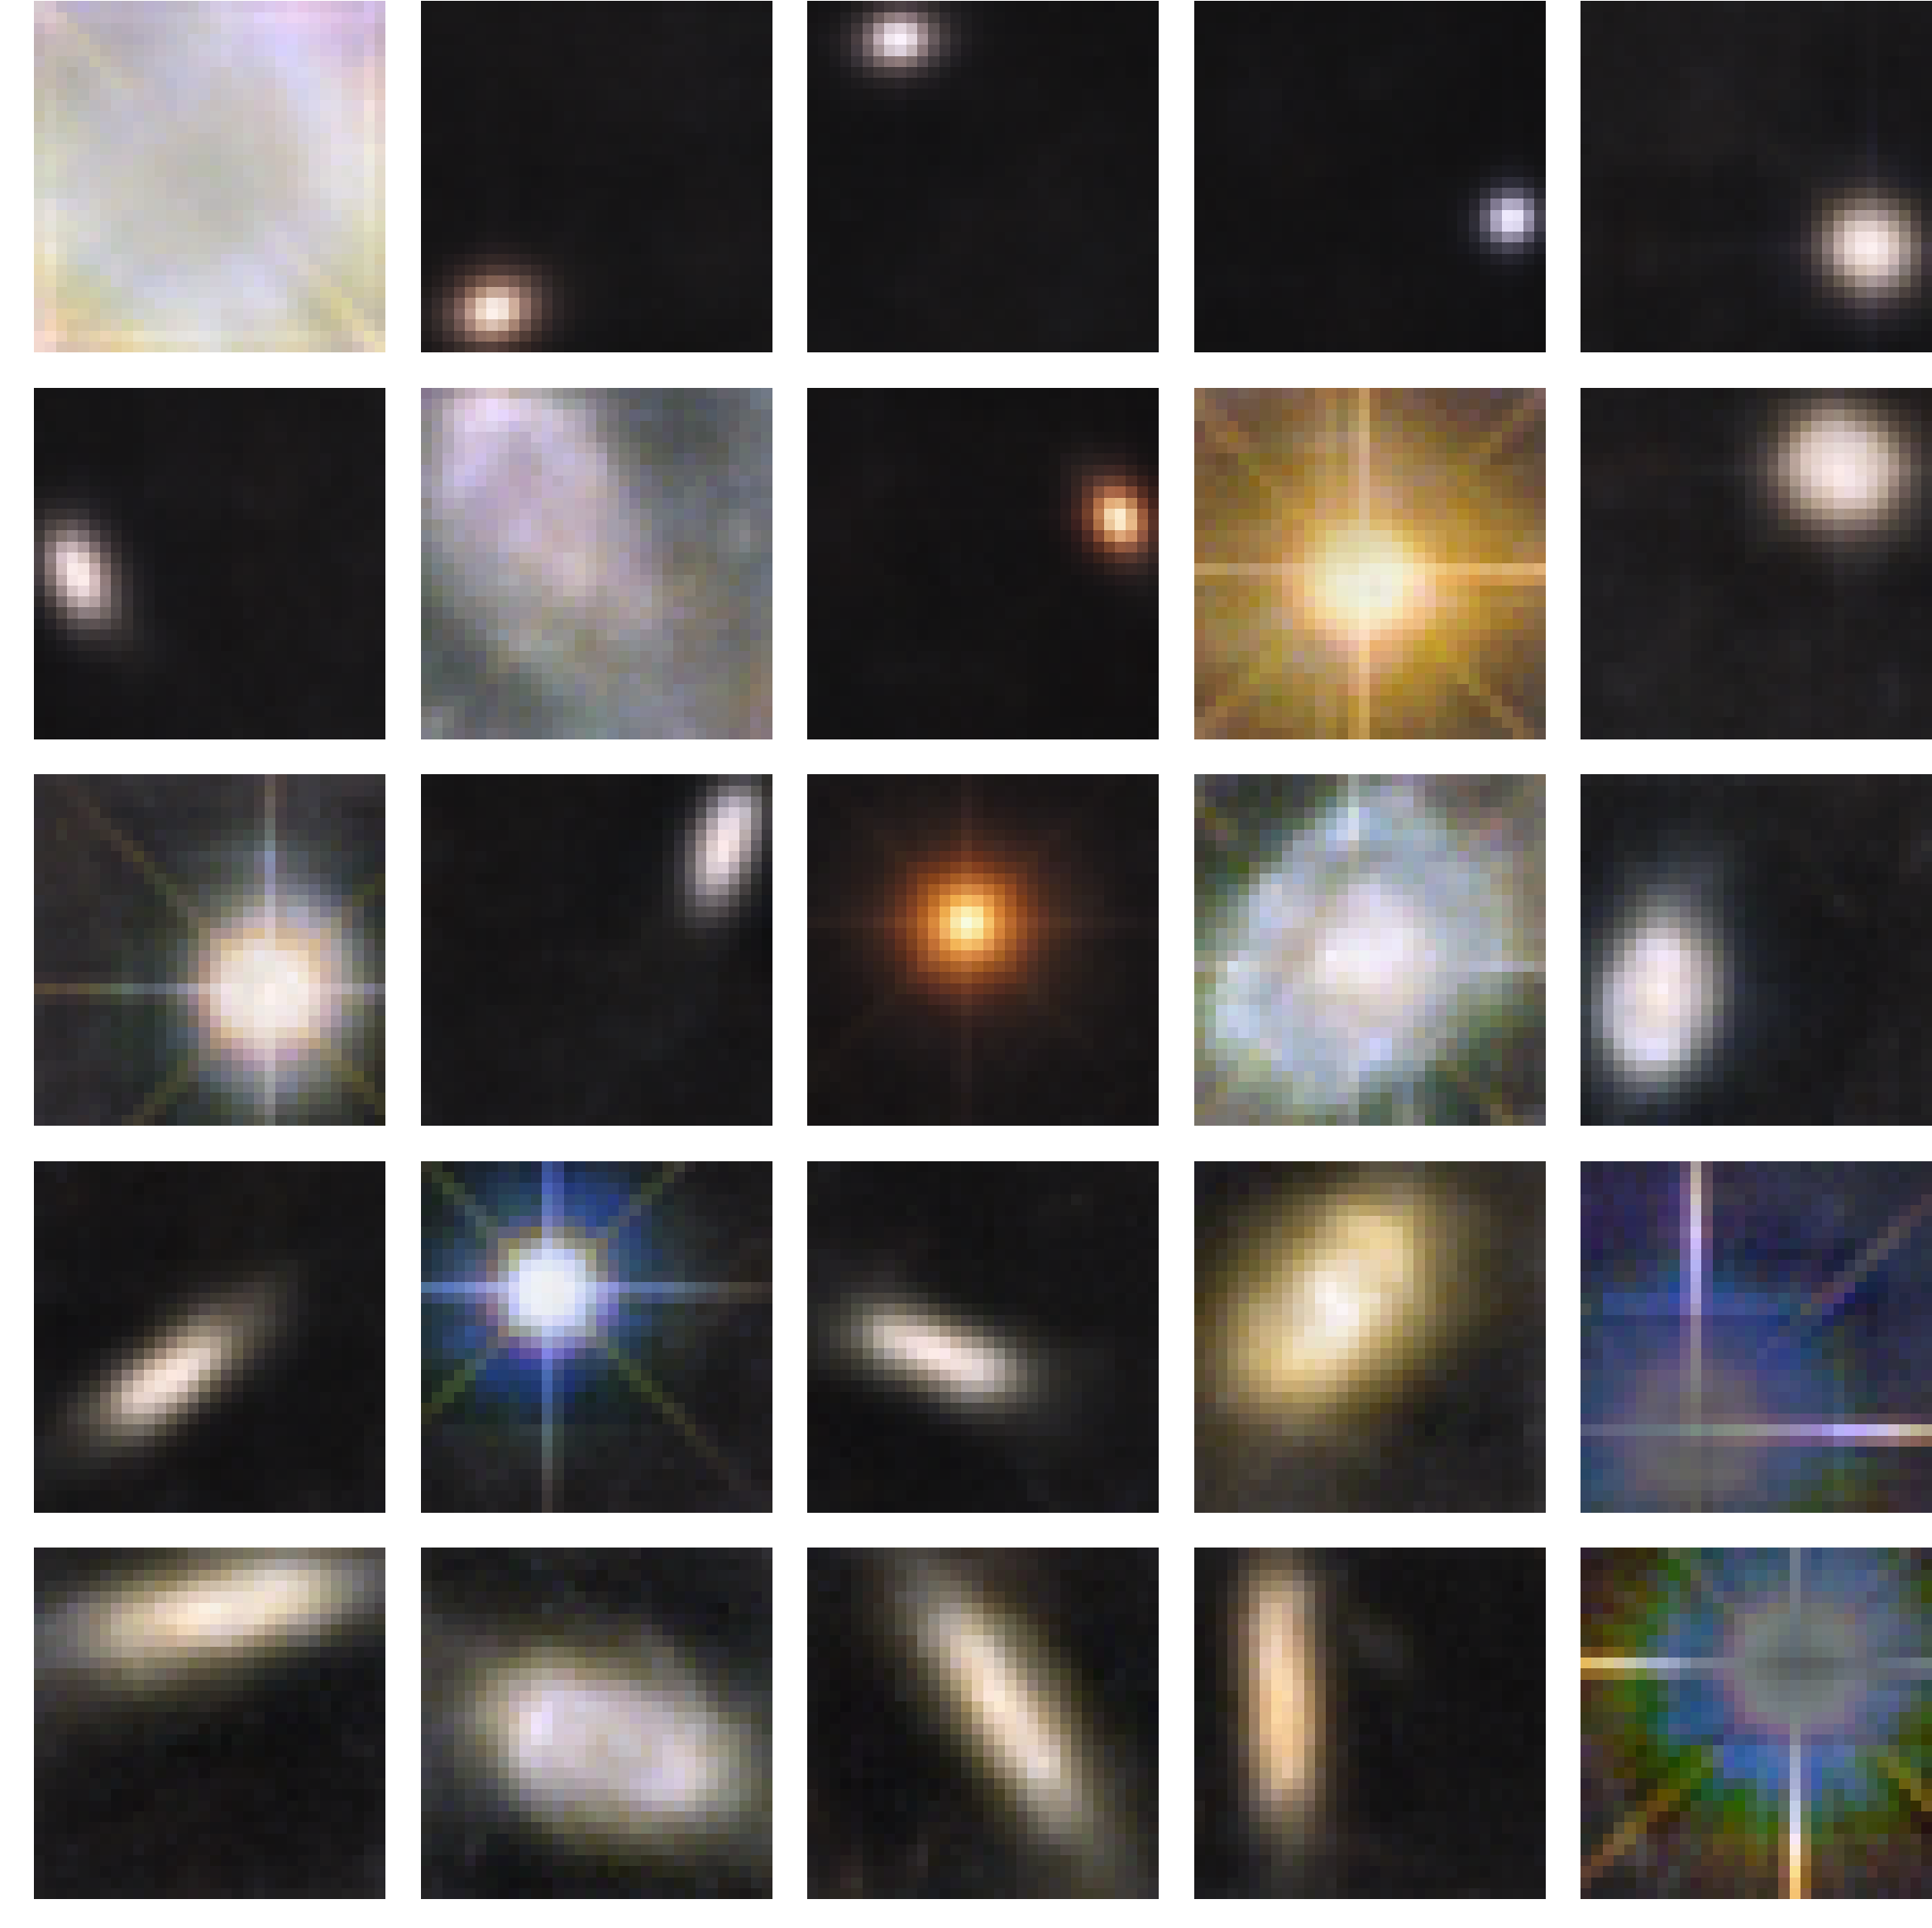
\includegraphics[width=.65\textwidth]{K25_L32_reg0,1_seed42_dicodile_Medium_dict}\\
    }
\end{center}

\end{frame}
}



%%%%%%%%%%%%%%%%%%%%%%%%%%%%%%%%%%%%%%%%%%%%%%%%
%   Conclusion
%%%%%%%%%%%%%%%%%%%%%%%%%%%%%%%%%%%%%%%%%%%%%%%%

\begin{frame}{Conclusion}

	\textbf{Take home message}\\[.5em]
	\begin{itemize}\itemsep.5em
        \item LGCD is a very efficient algorithm when working with CSC for long signals.
		\item Can be distributed efficiently for multi-dimensional signals,
		\item Good scaling properties with the number of workers $W$ used to distribute the algorithm.
	\end{itemize}
	\vskip1.5em
	
	\textbf{Ahead of us}\\[.5em]
	\begin{itemize}\itemsep.5em
		\item Extend this algorithm to local penalization such as Group LASSO.
        \item This algorithm could be used for algorithm such as MP for $\ell_0$ or $\ell_{0,\infty}$ penalties.
	\end{itemize}
\end{frame}

\biblio{}
\end{document}